\documentclass[../notes.tex]{subfiles}
\graphicspath{{\subfix{../img/}}}
\begin{document}

\part{ECE358: Foundations of Computing}

\marginnote{Taught by Prof. Shurui Zhou}

\section{Admin and Preliminary}

\subsection{Lecture 1}

Topics covered will include:
\begin{itemize}
	\item Graphs, trees
	\item Bunch of sorts
	\item Fancy search trees; red-black, splay, etc
	\item DP, Greedy
	\item Min span tree, single source shortest paths
	\item Maximum flow
	\item NP Completeness, theory of computation
	\item Blockchains??
	\item $ \Theta $ 
\end{itemize}

Solutions will be posted on the window of SF2001. Walk there and take a picture.

\subsubsection{Mark Breakdown}

\begin{table}[H]
	\centering
	\caption{Mark Breakdown}
	\begin{tabular}{|c|c|}
		\hline
		Homework x 5 & 25 \\
		Midterm (Open book) & 35 \\
		Final (Open book) & 40\\
		\hline
	\end{tabular}
\end{table}



\section{Complexities}


\subsection{Lecture 2}


This lecture we talked about big O notation. For notes on this refer to my tutorial notes for ESC180, ESC190: \href{https://github.com/ihasdapie/teaching/}{https://github.com/ihasdapie/teaching/}


\begin{definition}
	Big O notation (upper bound)

	$ g(n) $  is an asymptotic upper bound for $ f(n) $ if:

	\begin{equation}
		O(g(n)) = \left\{f(n): \exists \quad c, n_0 \quad s.t. \quad 0 \le  f(n) \le  c\cdot g(n), \forall n \ge  n_o \right\}
		\label{eq:358:bigOh}
	\end{equation}
\end{definition}

\begin{proof}

	\textbf{What is the big-O of $ n! $ }?
	\begin{equation}
			n! \le n \cdot n \cdot n \cdot  n \ldots n = n^n \Rightarrow n! \in O(n^n) 
	\end{equation}
\end{proof}



\begin{definition}
	Big $ \Omega $  notation (lower bound)

	$ h(n) $  is an asymptotic lower bound for $ f(n) $ if:
	\begin{equation}
		\Omega(h(n)) =  \left\{f(n): \exists \quad {c, n_0} > 0 \quad s.t. \quad 0 \le c \cdot h(n) \le  f(n), \forall n \ge  n_o \right\}
		\label{eq:358:bigOmega}
	\end{equation}
\end{definition}

\begin{proof}

	\textbf{Find $ \Theta $ for $ f(n) \sum^n_i i $}.

	For this we will employ a technique for the proof where we take the right half of the function, i.e. from $ \frac{n}{2} \ldots n $ and then find the bound

	\begin{equation}
		\begin{split}
			f(n) &= 1 + 2 + 3 \ldots + n \\
			 &\ge \lceil \frac{n}{2} \rceil + (\left\lceil \frac{n}{2} \right\rceil + 1) + (\left\lceil \frac{n}{2} \right\rceil + 2) + \ldots n \quad \text{$ n/2 $ times} \\
			 &\ge \left\lceil \frac{n}{2} \right\rceil +   \left\lceil \frac{n}{2} \right\rceil + \left\lceil \frac{n}{2} \right\rceil +  \ldots \left\lceil \frac{n}{2} \right\rceil \\
			 &\ge \frac{n}{2} \cdot \frac{n}{2} \\
			 &= \frac{n^2}{4} \\
		\end{split}
	\end{equation}

	And therefore for $ c = \frac{1}{4} $  and $ n = 1 $ , $ f(n) \in \Theta(n^2) $ 
	
	
\end{proof}



\begin{definition}
	Big $ \Theta $  notation (asymptotically tight bound)

	\begin{equation}
		\Theta(g(n)) = \left\{ f(n) : \exists \quad c_1 c_2, n_0 \quad s.t. \quad 0 \le  c_1 g(n) \le  f(n) \le  c_2 g(n), \forall n \ge  n_o   \right\}
		\label{eq:358:bigTheta}
	\end{equation}
\end{definition}

\begin{proof}
	Prove that 

	\begin{equation}
		\sum^n_{j=1} i^k = \Theta(n^{k+1})
	\end{equation}

	First, prove $ O(f(n)) = O(n^{k+1}) $ 

	\begin{equation}
		\begin{split}
			f(n) = \sum^n_{j=1} i^k &= 1^k + 2^k + \ldots n^k \\
			 &\le n^k + n^k + \ldots n^k  \\
			 &= n^{k+1} \\
		\end{split}
	\end{equation}


	Next, prove $ \Omega(f(n)) = \Omega(n^{k+1}) $ 

	\begin{equation}
		\begin{split}
			f(n) = \sum^n_{j=1} i^k &= 1^k + 2^k + \ldots n^k \\
			 &= n^k + (n_1)^k + \ldots 2^k + 1^k = \sum^n_{i=1} (n-i+1)^k \\
			 &\ge   \frac{n}{2}^k * n \ge \frac{n^{k+1}}{2^k} = \Omega(n^{k+1}) \\
		\end{split}
	\end{equation}

	Therefore $ f(n) = \Theta(n^{k+1}) $ 
\end{proof}

Note that we may not always find both a tight upper and lower bound so not all functions have a tight asymptotic bound.







\begin{theorem}
	\textbf{Properties of asymptotes:} 

	Note: $\land $ means AND

	\textbf{Transitivity} \mn{The following applies to $ O, \Theta, o, \omega $ }
	\begin{equation}
		(f(n) = \Theta(g(n)) \land g(n) = \Theta(h(n))) \Rightarrow f(n) = \Theta(h(n))
		\label{eq:358:asymptotic_transitivity}
	\end{equation} 


	\textbf{Reflexivity}\mn{The following applies to $ O, \Theta $ }
	\begin{equation}
		f(n) = \Theta(f(n))
		\label{eq:358:asymptotic_reflexivity}
	\end{equation}
	
	\textbf{Symmetry}
	\begin{equation}
		f(n) = \Theta(g(n)) \iff g(n) = \Theta(f(n))
		\label{eq:358:asymptotic_symmetry}
	\end{equation}
	

	\textbf{Transpose Symmetry}

	\begin{equation}
		\begin{split}
			 f(n) &= O(g(n)) \iff g(n) = \Omega(f(n))  \\
			 f(n) &= o(g(n)) \iff g(n) = \omega(f(n))  \\
		\end{split}
		\label{eq:358:asymptotic_transpose_symmetry}
	\end{equation}

\end{theorem}


Runtime complexity bounds can sometimes be used to compare functions. For example, $ f(n) = O(g(n)) $ is like $ a \le b $

\begin{itemize}
	\item $ O \approx \le $
	\item $ \Omega \approx \ge  $ 
	\item $ \Theta \approx \approx  $ 
	\item $ o \approx < $; an upper bound that is \textbf{not}  asymptotically tight
	\item $ \omega > $ a lower bound that is \textbf{not}  asymptotically tight
\end{itemize}

Note that there is no trichotomy; unlike real numbers where we can just do $ a<b $, etc, we may not always be able to compare functions.

\begin{figure}[H]
	\centering
	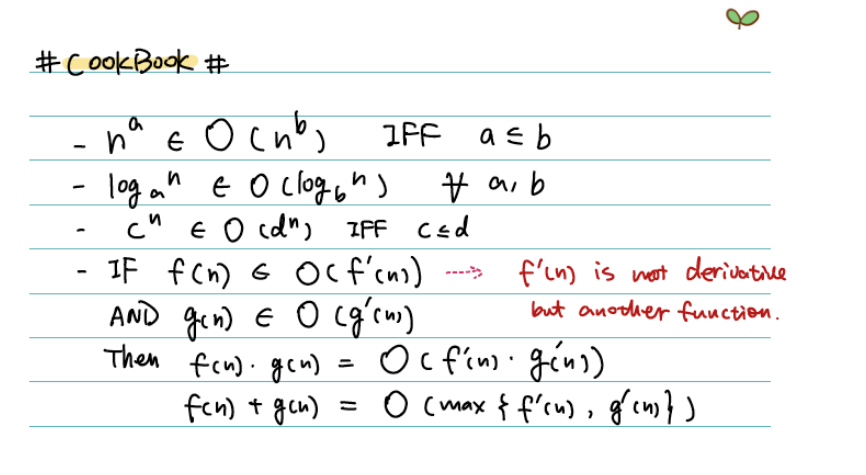
\includegraphics[width=0.8\linewidth]{img/image_2022-09-13-00-26-01.png}
	\caption{Complexity Cookbook}
	\label{fig:358:complexity_cookbook}
\end{figure}

\subsection{Lecture 3: Logs \& Sums}

\marginnote{
	Recall:
	\begin{equation}
		a = b^c \Leftrightarrow log_ba = c
	\end{equation}
}


\subsubsection{Functional Iteration}

$ f^{(i)}(n) $  denotes a function iteratively applied $ i $ times to value $ n $.

For example, a function may be defined as:
\begin{equation}
	f^{(i)}(n) = 
	\begin{cases}
		f(n) & \text{if } i = 0 \\
		f(f^{(i-1)}(n)) & \text{if } i > 0
	\end{cases}
	\label{eq:358:functional_iteration_1}
\end{equation}


Given \eqref{eq:358:functional_iteration_1} we see that 

\begin{enumerate}
	\item $ f(n) = 2n $ 
	\item $ f^{(2)}(n) = f(2n) = 2^2n$ 
	\item $ f^{(3}(n) = f(f^{(2)}(n)) = 2^3n$ 
	\vdots
	\item $ f^{(i)}(n) = 2^in $
\end{enumerate}


As an exercise we may look at an iterated logarithm function, 'log star`

\begin{equation}
	lg^*(n) = \min\{ i \ge  0 : lg^{(i)} n \le  1 \}
	\label{eq:358:iterated_logarithm}
\end{equation}

This describes the number of times we can iterate $ log(n) $ until it gets to $ 1 $ or smaller.

\begin{itemize}
	\item $ log^*2 = 1 $ 
	\item $ log^*4 = 2 = log^*2^2 = 1 + log^*2 = 2 $ 
		\vdots
	\item for practical reasons $ log^* $  doesn't really get bigger than $ 5 $. This is one of the slowest growing functions around.
\end{itemize}


\textbf{Summations \& Series} 

\begin{proof}

	Proof for a finite geometric sum:

	\begin{equation}
		\begin{split}
			\sum^n_{k=0} x^k &= S \\
			 S &= 1 + x + x^2 \ldots x^n  \\
			 xS &= x + x^2 + x^3 \ldots x^{n+1} \\
			 S &= \frac{1-x^{n+1}}{1-x} \\
		\end{split}
	\end{equation}
\end{proof}


\begin{equation}
	\sum^\infty_{i=1} x^i = \frac{1}{1-x} \quad \text{if } |x| < 1
	\label{eq:358:decreasing_geometric_series}
\end{equation}

\begin{equation}
	\sum^\infty_{k=0} kx^k = \frac{x}{(1-x)^2} \quad \text{if } |x| < 1
	\label{eq:358:geometric_series_2}
\end{equation}

\begin{proof}

	Begin by differentiating both sides over $ x $ 

	\begin{equation}
		\sum^\infty_{k=0} x^k = \frac{1}{(1-x)} \quad \text{if } |x| < 1
	\end{equation}

	\begin{equation}
		\sum^{\infty}_{k=0} kx^{k-1} = \frac{1}{(1-x)^2}
	\end{equation}

	And then multiply both sides by $ x $, therefore \eqref{eq:358:geometric_series_2} follows.
\end{proof}

\textbf{Telescoping Series} 

\begin{equation}
	\sum_{k=1}^{n} a_k - a_{k-1} = a_n - a_0
\end{equation}

\begin{proof}
	Write it out and cancel out terms
	\begin{equation}
		(a_1 - a_0) + (a_2 - a_1) \ldots (a_n - a_{n-1}) = a_n - a_0
	\end{equation}
	Therefore the sum telescopes
\end{proof}


Another telescoping series may be proved similarly:
\begin{equation}
	\sum^{n-1}_{k=1} \frac{1}{k(k+1)} \xrightarrow{math} \sum^{n-1}_{k=1} (\frac{1}{k} - \frac{1}{k+1}) 
	= 
	(1- \frac{1}{2}) + \ldots (\frac{1}{n-1} - \frac{1}{n}) = a_o - a_n
\end{equation}


\subsection{Lecture 4: Induction \& Contradiction}


\subsubsection{Induction}

The general steps for proving a statement by induction are:
\begin{enumerate}
	\item Basis
	\item Hypothesis
	\item Inductive step
\end{enumerate}

I.e. if the basis holds for some $ i $, i.e. $ 0, 1, 2, 3, 12, \ldots$ AND if we assume that the hypothesis holds for an arbitrary number $ k $, then we just need to prove that the inductive step follows, or that $ P(n+1) $ holds.

\begin{example}
	Prove that $ P(n) = 1+2+3+\ldots n = \frac{n(n+1)}{2} $ 
	\begin{proof}
		
	

	\begin{enumerate}
		\item Basis: $ P(0) = 0 = \frac{0(0+1)}{2} $
		\item Hypothesis (assume that it is true): $ P(k) = \frac{k(k+1)}{2} $
	\item Inductive step (need to prove $ P(k+1) = \frac{(n+1)(n+2)}{2} $ ): $ P(k+1) = \underbrace{1+2+\ldots+n}_{\frac{n(n+1)}{2}} + (n+1) = \ldots = \frac{n^2 + 3n + 2}{2} = \frac{(n+1)(n+2)}{2} $
	\end{enumerate}

	\end{proof}
	
\end{example}


\begin{example}
	Show that for any finite set $ S $, the power set $ 2^S $ has $ 2^{|S|} $ elements (that is, there are $ 2^{|S|} $ distinct subsets of $ S $  )\marginnote{The power set of a set $ S $ is the set of all subsets of $ S $ }

	\begin{proof}

		\begin{enumerate}
			\item Basis: 
				\begin{equation}
				n = 0, |S| = 0, |2^S| = 1 = 2^0 
				\end{equation}

				\begin{equation}
					n = 1, |S| = 1, |2^S| = 2 = 2^1
				\end{equation}
			\item Hypothesis: Assume that $ 2^S $ has $ 2^n $ elements when $ |S| = n $ 
			\item Inductive step: need to prove that when $ |S| = n+1, |2^S| = 2^{n+1} $ 

				Let $ B = S  \not \{a\}  $ for some $ a \in S $. 
				Now there are two types of subsets of $ S $; those that include $ a $ and those who do not include $ a $ 

				For subsets that do \textit{not} include  $ a $ , $ |2^{B}| = 2^{|B|} = 2^n $ , by the hypothesis.

				For subsets that do include $ a $, these sets are of size $ 2^B \cup \{a\}, which is  2^n  $ .

				Therefore the total number of subsets of $ S $ is $ 2^n + 2^n = 2^{n+1} $, as desired.
		\end{enumerate}
	\end{proof}
	
\end{example}

The same kind of argument can be applied to problems such as the \href{https://en.wikipedia.org/wiki/Tower_of_Hanoi}{Towers of Hanoi} and the tiling problem.


\subsubsection{Contradiction}
\begin{enumerate}
	\item Assume the theorem is false
	\item Show that the assumption is false (leads to a contradiction)
		\begin{itemize}
	\item Therefore the theorem is true
		\end{itemize}
\end{enumerate}

\begin{example}
	Prove that $ \sqrt{2}  $ is irrational
	\begin{proof}
		Assume that $ \sqrt{2}  $ is rational.

		Therefore we can write $ \sqrt{2}  $ as

		\begin{equation}
			\sqrt{2}  = \frac{a}{b}
		\end{equation}

		Where $ a, b $ \textbf{ have no common factors}.

		We can square both sides

		\begin{equation}
			2 = \frac{a^2}{b^2} \rightarrow a^2 = 2b^2
		\end{equation}

		Therefore $ a^2 $ is even. 

		Let $ a = 2c $ 

		\begin{equation}
			2^2 c^2 = 2b^2 \rightarrow b^2 = 2c^2
		\end{equation}

		Therefore $ b $ is even as well.

		This results in a contradiction since we assumed that $ a, b $ have no common factors, but our analysis shows that both would have to be even (and share a common factor of $ 2 $ ).
	\end{proof}
	
\end{example}


\subsection{Lecture 5: recurrences}
Many recursive algorithms can be thought of as a divide-and-conquer approach where we break the problem into subproblems that are similar to the origianl but smaller in size, solve them resurisively, then combine them to create a solution to the original problem.


\begin{definition}
	A recurrence is a function defined in terms of:
	\begin{itemize}
		\item 1+ base cases
		\item Itself, with smaller arguments
	\end{itemize}
\end{definition}

For example, finding a Fibonacci number is a recurrence;

$ T(n) = T(n-1) + T(n-2) $ with some base cases.



\begin{example}
	\textbf{Mergesort} 

	Sorting $ [3,1,7,5] $ 

	\begin{enumerate}
		\item Divide: break into partitions: $ [[3, 1], [7, 5]] $ 
		\item Sort partitions: $[[1, 3], [5, 7]] $ 
		\item Create result array
		\item Compare: have two pointers to front of array
			\begin{itemize}
				\item compare 1, 5. 1 is smaller; $ result = [] \leftarrow 1 $ 
				\item Move ptr to left array (1, 3) ahead one. Compare 3, 5. 3 is smaller, so $ result = [3] \leftarrow 3 $ 
				\item One of the arrays is now empty so we can just append the rest
			\end{itemize}
		\item $ result = [1, 3, 5, 7] $ 
	\end{enumerate}
\end{example}


\begin{definition}
	Pseudocode for mergesort is given by:

	\begin{listing}[H]
	\begin{minted}{text}
	mergesort(A, p, r)
		if p < r
			q = [(p+r)/2]
			mergesort(A, p, q)  // N/2
			mergesort(A, q+1, r)  // N/2
			merge(A, p, q, r) // merge the sorted subarrays
	\end{minted}
	\end{listing}

	This mergesort partitions in half each time\mn{binary partitioning(?)}.

	In the worst case we will compare $ N-1 $ times, so $ O(N) $ worst case.

	Proving that merge sort is $ \Omega(N) $ 
	\marginnote{Here we're discussing not time complexity but rather the number of times we call mergesort}
	
\end{definition}

How much time does MergeSort take?


The time of mergesort is defined recursively as:
\begin{equation}
	T(N) = \begin{cases}
		O(1) & n = 1 \\
		T(N) = 2T(\frac{N}{2} + \Theta(N)
	\end{cases}
\end{equation}

\marginnote{Note that $ \Theta(N) $ is for the merge operation }

More generally we can find the runtime of a recurrence algorithm via
\begin{itemize}
	\item Recurrence trees
	\item Substitution
	\item Master theorem
\end{itemize}


\subsubsection{Recurrence Trees}
\begin{example}
Recurrence trees can be used to find the time complexity of mergesort.
\begin{figure}[H]
	\centering
	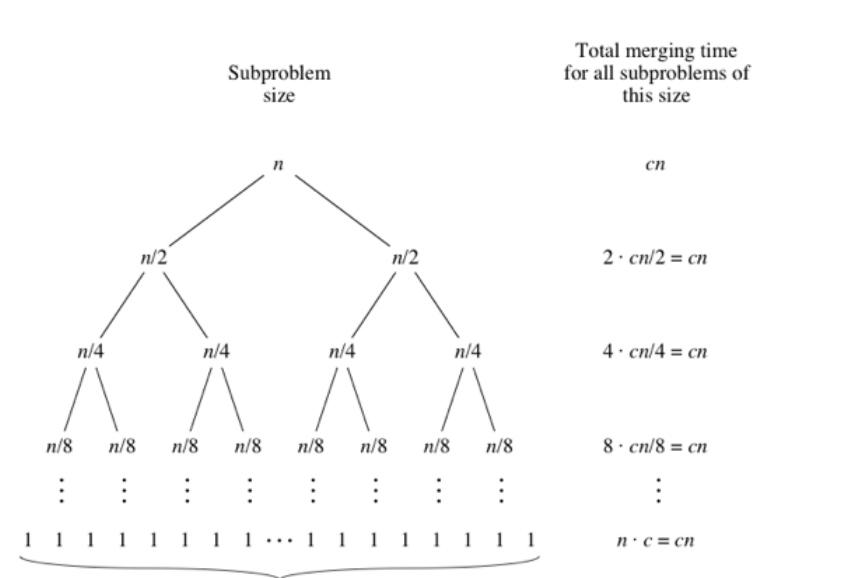
\includegraphics[width=0.8\linewidth]{img/image_2022-09-19-12-26-07.png}
\end{figure}

The height of the tree is $ \log N$ 

The total cost is the total cost per level times the number of levels, which is 

\begin{equation}
	N \cdot  logN
\end{equation}

So the complexity is $ O(N\log N) $ 
	
\end{example}

\subsubsection{Substitution}

\begin{enumerate}
	\item Guess the answer
	\item Apply induction
\end{enumerate}


\begin{example}
	Determine an asymptotic upper bound on $ T(n) = 2T(\left\lfloor \frac{n}{2} \right\rfloor ) + \Theta(n)$ 
	\begin{proof}

		This expression can be simplified since we don't care too much about floors or ceilings for asymptotic behaviour.

		\begin{equation}
			T(n) = 2T(\frac{n}{2}) + N
		\end{equation}

		Let's guess that the upper bound is $ O(n\log n) $ 

		Then, we need to prove that $ T(n) < C \cdot n \log n$  for some $ C > 0 $. Let's apply induction.

		\begin{enumerate}
			\item Basis: this is tricky since if $ n =1  $ we end up with $ T(1) \le  C \cdot 1 \cdot \log 1 = 0$ which cannot hold since that would just not make sense. Instead, observe that $ T(1) = 1 $, $ T(2) = 2T(1) + 2 = 4 $, $ T(3) = 2T(1) + 3 = 5  $, $ T(4) = 2T(2) + 4  \ldots$.

				So $ T(n) $ is therefore independent of $ T(1) $, so we can use two bases, $ T(2),T(3)$. Since $ T(2) \le  C * 2 \log 2 = 2C$, $ T(3) \le C \cdot \log  $ 
			\item Hypothesis: Assume that the upper bound holds for all possible $ m < n$, let $ m = \left\lfloor \frac{n}{2} \right\rfloor$ . This yields $ T(\frac{n}{2}) \le C \cdot  \left\lfloor \frac{n}{2} \right\rfloor \cdot  \log \left\lfloor \frac{n}{2} \right\rfloor $ 
			\item Inductive step: substitute hypothesis into recurrence yields 

				\begin{equation}
				 T(N) \le C \cdot ( C \cdot \left\lfloor  \frac{N}{2} \right\rfloor \cdot  \log \left\lfloor \frac{N}{2} \right\rfloor + N  = c N\log N - (1-c)N \le Cn\log n
				\end{equation}
		\end{enumerate}
		
	\end{proof}

	A few pitfalls to avoid is guessing $ T(n) = O(n) = c \cdot  n $ and so forth we would get

	\begin{equation}
		T(N) \le  2 C \cdot  \left\lfloor \frac{n}{2} \right\rfloor + n = cn+n = (c+1)n
	\end{equation}

	This would be wrong since we cannot change the constant to $ c+1 $; we have to prove it with exactly the hypothesis given.
	
\end{example}

\subsubsection{Master Theorem}

\marginnote{Proof is out of scope for the course}
\begin{definition}
	The master method applies to recurrences of the form 

	\begin{equation}
		T(n) = a T(\frac{n}{b}) + f(n) \qquad \text{where } a \ge 1, b >  1, f  \text{asymptotically positive}
	\end{equation}

	It distinguishes 3 common cases b comparing $ f(n)  $  with $ n^{\log_ba}$ 

	\begin{enumerate}
		\item If $ f(n) = O(n^{\log_ba - \varepsilon}) $ for some $ \varepsilon > 0 $, then $ T(n) = \Theta(n^{log_ba}) $ 
		\item If $ f(n) = \Theta(n^{\log_ba }) $, then $ T(n) = \Theta(n^{log_ba}\log n) $ 
		\item If $ f(n) = \Omega(n^{\log_ba + \varepsilon}) $ for some $ \varepsilon>0 $ and $ af(\frac{n}{b}) \le  c f(n) $ for some $ c < 1$, then then $ T(n) = \Theta(f(n)) $ 
	\end{enumerate}
\end{definition}


There are a few technicalities to be a ware of. 
In each example we compare $ f(n) $ with $ F = n^{\log_ba} $ and take the larger of each as the solution the recurrence. 
For the first case we note that $ f(n) $ must be \textit{polynomially} smaller than $ F $; i.e. it must be asymptotically smaller than $ F $ by some factor of $ n^\varepsilon $.
In the third case $ f(n)  $ must be greater than $ F $ as well as being polynomially larger and satisfy the regularity condition $ af(\frac{n}{b}) \le cf(n)$.
There are areas where the master theorem does not cover, for example a gap between cases 1, 2 where $ f(n) > F $ but is not polynomially larger. If $ f(n)  $ falls in one of these gaps or the regularity condition does not hold, the master method cannot be used to solve the recurrence.


\begin{example}

	What is the closed form of $T(n) = T(\frac{2n}{3}) + 1$ ?

	\begin{proof}
		a = 1, b = 2/3, f(n) = 1.

		\begin{equation}
			\log_ba = \log_{\frac{2}{3}} 1 = 0 
		\end{equation}

		\begin{equation}
			f(n) = \Theta(n^0)
		\end{equation}

		So
		\begin{equation}
			T(n) = O\log(n)
		\end{equation}
		
	\end{proof}
	


	
\end{example}








\subsection{Lecture 6}

\subsubsection{Graphs}

\begin{definition}
A \textbf{graph} is a data structure comprised from set of vertices $ V $ and a set of edges $ E $, where each edge connects a pair of vertices.
A \textbf{directed graph (digraph)} is a graph where edges $ E $ have a \textit{direction}, i.e. an edge $ (u,v) $ is different from $ (v,u) $.
Conversely, an \textbf{undirected graph} is a graph where edges $ E $ do not have a direction.
\begin{figure}[H]
	\centering
	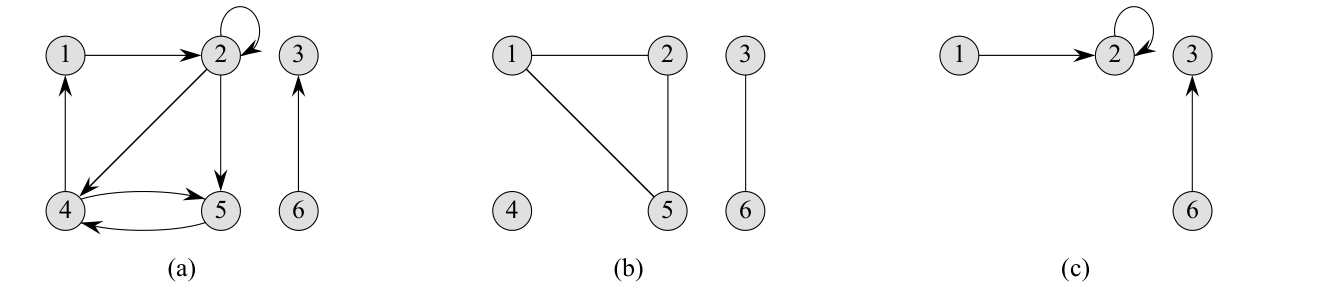
\includegraphics[width=0.8\linewidth]{img/image_2022-09-22-00-05-04.png}
	\caption{(a) directed graph, (b) undirected graph, (c) a subgraph of (a)}
\end{figure}

\end{definition}

Some conventions:

\begin{itemize}
	\item Edges are denoted by $ (u,v) $\mn{not $ \{u, v\} $  } where $ u,v \in V $
	\item If $ (u,v)$ is a edge in a directed graph, then $ (u,v) $ is incident from or leaves $ u $, and is incident to or enters $ v $ 
	\item If $ (u,v) $ is a edge a graph, then $ u$ , $ v $ are adjacent
	\item The \textbf{degree} of a vertex is the number of edges incident to it
	\item A \textbf{path} is a sequence of vertices $ (v_0, v_1, \ldots v_k) $ from from vertex to another such that each vertex is incident\mn{with the exception of start/end vertices} to the ones prior and after.
		\begin{itemize}
			\item If there exists a path from $ a $  to $ b $ then $ b $ is \textbf{reachable} from $ a $ and $ a $
			\item A path is \textbf{simple}  if no vertex is repeated
			\item A path forms a cycle if the first and last vertices are the same
		\end{itemize}
	\item A directed graph with no self-loops is \textbf{simple} 
	\item A graph with no simple cycles is acyclic
	\item An undirected graph is \textbf{connected} if there exists a path between any two vertices
	\item A directed graph is \textbf{strongly connected} if every vertex is reachable from every other vertex
	\item Two graphs $ V, V' $  are \textbf{isomorphic} if there exists a bijection\mn{$ f: V \to V' $, i.e. we can relabel the vertices of $ V $ to be those of $ V' $ and the two graphs would be identical   } between the vertices of the two graphs such that the edges are preserved
	\item Given graph $ G $,  $ G' = (V', E') $ is a \textbf{subgraph}  of $ G $  if $ V' \subseteq V $ and $ E' \subseteq E $
	\item Given a set $ V' \subseteq V $, the subgraph of $ G $ \textbf{induced} by $ V' $ is the graph $ G' = (V', E') $ where $ E' = \{ (u,v) \in E | u,v \in V' \} $
	\item Given an undirected graph, the \textbf{directed version} of $ G $ is $ G = (V, E') $  where $ (u,v) \in E' $ if and only if $ (u,v) \in E $. In other words we replace all undirected edges and replace them with their directed counterpart.
	\item The corollary can be applied to a directed graph to get the \textbf{undirected version} of $ G $.
	\item A \textbf{neighbor} of $ u $ in a directed graph is any vertex $ v $ such that $ (u,v) \in E $ where $ E $ is the set of edges for the undirected counterpart of the graph
	\item A \textbf{complete} graph is a graph where every pair of vertices are connected by an edge
	\item A \textbf{bipartite graph} is an undirected graph $ G $  in which it's $ V $ can be partitioned into two disjoint sets $ V_1, V_2 $ such that every edge $ (u,v) \in E $ connects a vertex in $ V_1 $ to a vertex in $ V_2 $ or vice-versa
	\item An acyclic undirected graph is a \textbf{forest}
	\item A connected acyclic undirected graph is a \textbf{free tree}. 
		\begin{itemize}
			\item A directed acyclic graph is often termed a DAG
		\end{itemize}
	\item A multi-graph is a graph where edges can be repeated and self-loops are allowed
	\item A hyper-graph is a graph where edges can connect more than two vertices
	\item The \textbf{contraction} of an undirected graph $ G $ by an edge $ e = (u,v) $ is a graph $ G' $  where $ V' = V - \{u,v\} \cup \{x\} $, where $ x $ is a new vertex. Then, for each edge connected to $ u, v$ the edges are deleted and then reconstructed with $ x $, effectively 'contracting` $ u ,v $  into a single vertex
\end{itemize}

In code graphs are commonly represented as adjacency lists or adjacency matrices. 
This was covered in ESC190, but for reference:

\begin{figure}[H]
	\centering
	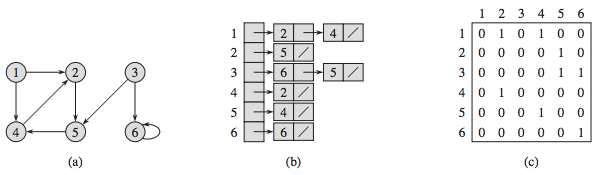
\includegraphics[width=0.8\linewidth]{img/image_2022-09-22-00-29-19.png}
\end{figure}

\begin{table}[H]
	\centering
	\caption{Time complexities of graph representations}
	\begin{tabular}{c|c|c|}
		\hline
		& adjacency list & matrix  \\
		Time & $ O(n) $ & $O(1)$ \\ 
		Memory & $ O(E) $ & $ O(n^2) $ 
	\end{tabular}
\end{table}












\subsubsection{Trees}

A \textbf{tree} is a common and useful subset of graphs
\begin{figure}[H]
	\centering
	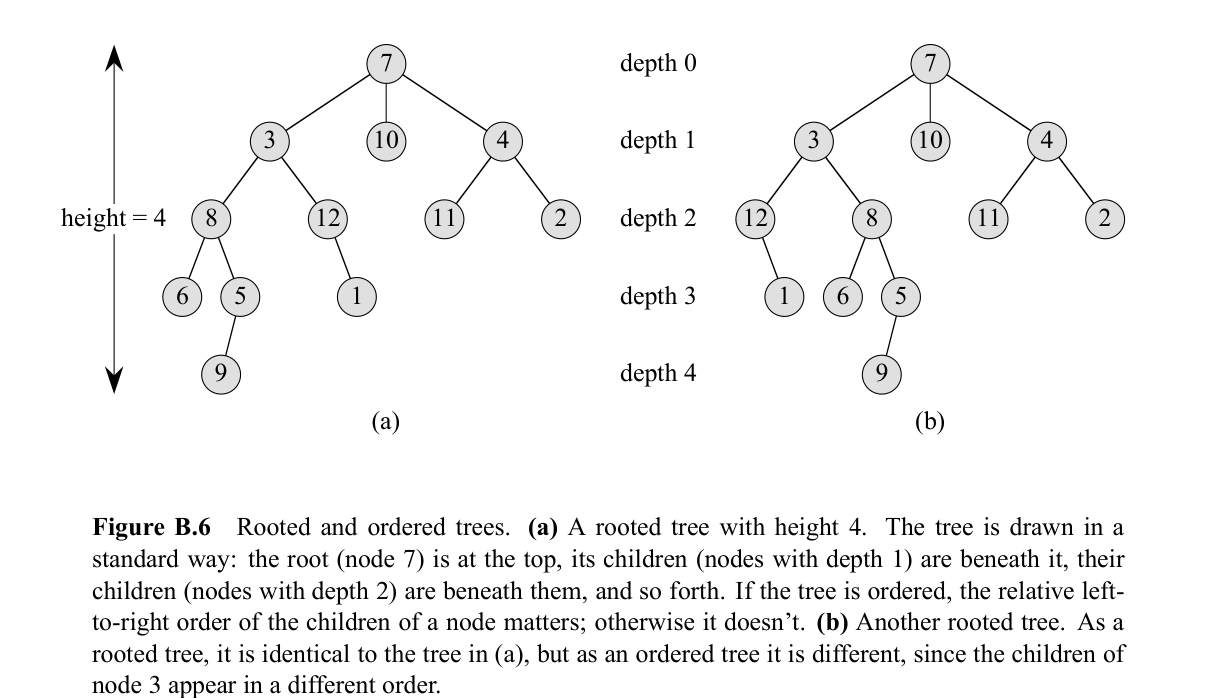
\includegraphics[width=0.8\linewidth]{img/image_2022-09-22-00-39-29.png}
\end{figure}
\begin{definition}
	A tree is a common subset of graphs, i.e. ones that are \textbf{connected, acyclic, and undirected}.
	This gives a few useful properties, i.e. the existence of a \textit{root} node, the parent-child relationship, and the existence of a unique path between any two nodes.
\end{definition}

Some conventions for trees

\begin{itemize}
	\item Depth of node: length from root to node
	\item Height length of longest path from node to leaf
	\item Degree of node: number of children. Binary trees have degree 2, n-ary tree has degree n
\end{itemize}

\begin{theorem}
	All of the following statements are equivalent for a tree $ T = (V, E) $:

	\begin{enumerate}
		\item $ \forall v \in V, v $ is a tree; all nodes in a tree are trees unto themselves.
		\item Every two nodes are connected by a unique path
		\item $ T $ is connected by if any edge is removed the resulting graph is disconnected
			$ T $ is connected and $ |E| = |V| - 1 $   
			$ T $ is acyclic and $ |E| = |V| - 1 $   
			$ T $ is connected but if a edge is added the resulting graph has a cycle
	\end{enumerate}



\end{theorem}






\subsection{Lecture 7, 8: Probability and Counting}

Most of the probability stuff is review from ECE286 so I'll be omitting most notes.


\begin{definition}
	Probability distribution $ Pr \left\{  \right\}  $: mapping from events of $ S $ to real numbers where

	\begin{enumerate}
		\item $ Pr \left\{ \emptyset \right\} = 0 $
		\item $ Pr \left\{ A \right\} \ge  0  \forall A \in S $
		\item $ Pr \left\{ S \right\} = 1 $
		\item $ Pr \left\{ A \cup B \right\} = Pr \left\{ A \right\} + Pr \left\{ B \right\} \forall A, B \in S $
	\end{enumerate}
\end{definition}
\marginnote{The complement of an event $ A $ is $ \overline{A} = S-A $, and the probability is $ Pr \left\{ \overline{A} \right\} = 1- Pr \left\{ A \right\}  $  } 

For any two events $ A, B $ we can define the triangle inequality
\begin{definition}
	$ Pr \left\{ A \cup B \right\} \le Pr \left\{ A \right\} + Pr \left\{ B \right\} $
\end{definition}


\begin{definition}
	Baye's thereom


	\begin{equation}
		Pr \left\{ A \mid B \right\} = \frac{Pr \left\{ B \mid A \right\} Pr \left\{ A \right\}}{Pr \left\{ B \right\}}
		= \frac{Pr \left\{ A \right\} Pr \left\{ B | A \right\} }{Pr \left\{ A \right\} Pr \left\{ B | A \right\} + Pr \left\{ \overline{A} \right\} Pr \left\{ B | \overline{A} \right\} }
	\end{equation}
	
\end{definition}


The expected value of a random variable is 

\begin{equation}
	E[X] = \int_{-\infty}^{\infty} x Pr \left\{ X = x \right\} dx
\end{equation}

And in the discrete case,
\begin{equation}
	E[X] = \sum_{x \in \mathbb{Z}} x Pr \left\{ X = x \right\}
\end{equation}


The variance is 

\begin{equation}
	Var[X] = E \left\{ \left( X - E[X] \right)^2 \right\} = E[X^2] - E^2[X]
\end{equation}

\marginnote{The \textbf{standard deviation, $ \sigma $, } is the positive square root of the variance.}




\subsection{Lecture 9: Heapsort}

Heapsort is a sorting algorithm that runs in $ O(nlog(n)) $ and sorts its elements in place by leveraging a \textit{heap}.
\marginnote{This should be review from ESC190}

\begin{definition}
A heap is a data structure that satisfies the \textit{heap property}. For a max heap, the value of a mode is at most the value of its parent and vice-versa for a min-heap. Heaps are commonly used to implement a priority queue because it offers a \texttt{pop\{min, max\}} operation in $ O(1) $ time and insertion in $ O(log(n)) $ time. Another reason for its use is it's ability to be represented as an array with \texttt{Parent(i) = floor(i/2)}, \texttt{Left(i) = 2i}\texttt{Right(i) = 2i+1} 

\end{definition}


The \texttt{MAXHEAPIFY} method is used to coerce heaps back into fulfilling the heap property by `bubbling down' nodes until the heap property is satisfied.
The intuition for this is that as long as the heap property is not satisfied\sn{which we can tell by looking at the node's children}, node $ i $ is exchanged for the largest of its' children. Since the heap property is now satisfied for $ i $ but not necessarily its' children, this heapify operation is then recursively called on the larger of $ i $'s children.

\begin{listing}[H]
\begin{minted}{text}
MAXHEAPIFY(A, i)
	l = LEFT(i)
	r = RIGHT(i)
	if l <=A.size and A[l] > A[i]
		largest = l
	else largest = i
	if r <= A.size and A[r] > A[largest]
		largest = r
	if largest != i
		swap A[i], A[largest]
		MAXHEAPIFY(A, largest)
\end{minted}
\end{listing}


The child sub-trees can have size of at most $ \frac{2n}{3} $ and so we can describe MAXHEAPIFY by the recurrence relation

\begin{equation}
	T(n) = \le  T(\frac{2n}{3}) + \Theta(1)
\end{equation}





This heapify operation can then be used to build a max heap from an array by calling heapify on all nodes that are not leaves. This is done by starting at the last node that has children and calling heapify on it. This is repeated until the root is reached. It can likewise be used to sort an array.



\begin{listing}[H]
\begin{minted}{text}
HEAPSORT(A)
for i = A.length -> 2,
	swap A[1], A[i]
	A.heapsize = A.heapsize - 1
	HEAPIFY(A, 1)
\end{minted}
\end{listing}



\subsection{Placeholder for Quick, counting, selection, and radix sort}

I'm going to skip these since these are fairly trivial and easily found online. I also didn't go to class.

\subsection{BSTs}


\subsection{Amortized Analysis}
\begin{definition}

	\begin{itemize}
		\item \textbf{Average cost}: mean across all inputs

			\begin{equation}
				\frac{1}{T-0} \int_{0}^{T} c(x) dx 
			\end{equation}
			
		\item \textbf{Expected cost}: expectation over all inputs w.r.t a probability distribution

			\begin{equation}
				\int_{0}^{T}   p(x) c(d) dx
			\end{equation}
			
		\item \textbf{Amortized Cost}: average cost over a \textit{sequence} of operations

			\begin{equation}
				\frac{1}{n} \sum_{i=1}^{n} c(\frac{1}{n})
			\end{equation}
	\end{itemize}

\end{definition}

The aggregate analysis method is simple and is as follows

\begin{enumerate}
	\item Given a function or operation $ f(x) $ and a sequence $ \left\{ x_1, x_2, \ldots x_n \right\}  $
	\item Determine the total cost of the sequence $ \sum_{i=1}^{n} c(x_i) \equiv T(n) $
	\item The amortized cost is $ \frac{T(n)}{n} $
\end{enumerate}

The complicated but more powerful way to deal with this is the accounting method.


\begin{enumerate}
	\item Declare a cost $ \hat{c} $ for each operation/function call
	\item Describe a procedure for how the cost will be allocated
	\item Assert a credit invariant, i.e. that the credit in an object must be greater than or equal to 0
	\item Prove the credit invariant
	\item Using the credit invariant argue why the credit never goes negative
	\item The amortized cost is $ O(\hat{c}) $
\end{enumerate}



\subsection{Skewed Heaps}




% 358 END
\end{document}
